
\setcounter{chapter}{4}
\chapter{First and Second Order Systems}

\begin{quote}
\textit{``The fundamental frequencies of a vibrating system are as characteristic of that system as the features of a face are characteristic of an individual.''} --- Lord Rayleigh, Theory of Sound (1877)
\end{quote}

\vspace{1em}

The study of first and second order systems forms the cornerstone of control systems engineering. These canonical forms appear with remarkable universality across disciplines---from the gentle swing of a pendulum to the complex dynamics of spacecraft attitude control, from the absorption of medication in the bloodstream to the oscillations of bridges in the wind. Understanding these fundamental building blocks provides engineers with powerful tools to analyze, predict, and design the behavior of far more complex systems.

This chapter develops the complete mathematical framework for first and second order systems, traces their historical origins, and connects theory to modern applications. We begin with the rich history that led to our current understanding, proceed through rigorous mathematical derivations, and conclude with hands-on experiments that bring these concepts to life.

%=============================================================================
\section{Historical Motivation: The Quest to Understand Oscillation}
%=============================================================================

The mathematical description of first and second order systems emerged from centuries of scientific inquiry into the fundamental nature of motion, vibration, and response to disturbance. The journey from empirical observation to precise mathematical characterization represents one of the great intellectual achievements of classical physics and engineering.

%-----------------------------------------------------------------------------
\subsection{Lord Rayleigh and the Theory of Sound (1877)}
%-----------------------------------------------------------------------------

\begin{historicalbox}[The Birth of Systematic Vibration Analysis]
John William Strutt, the 3rd Baron Rayleigh (1842--1919), published his monumental two-volume treatise \textit{``The Theory of Sound''} in 1877--1878. This work systematically applied the methods of mathematical physics to the analysis of vibrating systems and acoustic phenomena.
\end{historicalbox}

Rayleigh's contribution was revolutionary in its scope and rigor. While earlier scientists such as Daniel Bernoulli, Leonhard Euler, and Jean-Baptiste Fourier had made significant contributions to understanding vibration and wave phenomena, Rayleigh synthesized these disparate results into a unified framework. His treatise established the fundamental principle that complex vibrating systems could be understood as combinations of simpler modes, each characterized by its natural frequency and damping.

The second-order differential equation emerged as the canonical description of a single vibrational mode:
\begin{equation}
m\frac{d^2x}{dt^2} + c\frac{dx}{dt} + kx = F(t)
\label{eq:rayleigh_oscillator}
\end{equation}

Rayleigh recognized that this equation described not just mechanical oscillators, but a vast class of physical phenomena. He introduced the concept of the \textit{quality factor} $Q$, related to what we now call the damping ratio, to characterize how sharply tuned a resonant system was. His analysis of coupled oscillators laid the groundwork for understanding multi-degree-of-freedom systems and modal analysis.

Perhaps most significantly, Rayleigh understood that the \textit{poles} of a system---the roots of the characteristic equation---completely determined the qualitative behavior of the response. An oscillator with complex poles would exhibit sinusoidal behavior; one with real poles would show purely exponential decay. This insight, formalized mathematically in terms of the Laplace transform decades later, remains the central organizing principle of linear systems theory.

%-----------------------------------------------------------------------------
\subsection{Seismograph Development and the Need for Instrument Theory (1880s)}
%-----------------------------------------------------------------------------

The 1880s witnessed rapid development in seismology, driven by devastating earthquakes in Japan, Italy, and California. Scientists and engineers faced a fundamental challenge: how could they design instruments to faithfully record ground motion without the instrument's own dynamics distorting the measurement?

\begin{historicalbox}[The Seismograph Problem]
John Milne, James Ewing, and Thomas Gray, working in Japan during the 1880s, developed increasingly sophisticated seismographs. Their instruments were essentially mass-spring-damper systems, and they quickly realized that the recorded signal was a \textit{convolution} of the ground motion with the instrument's impulse response.
\end{historicalbox}

This realization forced seismologists to develop rigorous theories of second-order system response. If the seismograph had natural frequency $\omega_n$ and damping ratio $\zeta$, the behavior depended critically on the relationship between earthquake frequency and instrument frequency. For ground oscillations at frequencies much \textit{lower} than $\omega_n$, the seismograph mass would move with the ground, providing a displacement measurement. Conversely, for ground oscillations at frequencies much \textit{higher} than $\omega_n$, the mass would remain stationary while the frame moved, effectively measuring acceleration. For frequencies \textit{near} $\omega_n$, resonance would amplify or distort the signal, making interpretation difficult.

The damping ratio became critical: too little damping and the instrument would ring excessively after each seismic event; too much damping and the instrument would be sluggish and miss rapid changes. Through empirical study and theoretical analysis, seismologists determined that $\zeta \approx 0.7$ (critically damped to slightly underdamped) provided the best compromise---a finding that would later influence control system design across all disciplines.

Emil Wiechert's inverted pendulum seismograph of 1904 exemplified the mature understanding of second-order system theory. By carefully choosing the natural frequency and damping ratio, Wiechert created instruments capable of recording earthquake waves that had traveled thousands of kilometers through the Earth.

%-----------------------------------------------------------------------------
\subsection{Automotive Suspension Design (1920s--1930s)}
%-----------------------------------------------------------------------------

The rapid proliferation of automobiles in the early twentieth century created an urgent engineering challenge: how to isolate passengers from road irregularities while maintaining vehicle stability and control. This problem is fundamentally one of second-order system design.

\begin{historicalbox}[The Suspension Trade-off]
Early automobiles used simple leaf spring suspensions inherited from horse-drawn carriages. As speeds increased, engineers discovered that comfortable ride and precise handling were conflicting objectives---a trade-off that could only be optimized through careful control of damping ratio and natural frequency.
\end{historicalbox}

The automobile suspension system is a classic second-order system characterized by three fundamental parameters: the mass $m$ representing the sprung mass (vehicle body), the spring constant $k$ provided by coil springs, leaf springs, or torsion bars, and the damping coefficient $c$ provided by hydraulic shock absorbers.

The natural frequency $\omega_n = \sqrt{k/m}$ determines how quickly the suspension responds to bumps. Human comfort studies during this era established that natural frequencies between 1--1.5~Hz were optimal for passenger comfort, matching the natural frequency of the human body in seated position.

The damping ratio $\zeta = c/(2\sqrt{km})$ became the primary design variable for balancing competing objectives:

\begin{center}
\begin{tabular}{lll}
\toprule
\textbf{Damping Ratio} & \textbf{Ride Quality} & \textbf{Handling} \\
\midrule
$\zeta < 0.3$ & Very soft, floaty & Poor body control \\
$\zeta \approx 0.3$--$0.4$ & Comfortable (luxury cars) & Acceptable \\
$\zeta \approx 0.5$--$0.7$ & Firm but controlled & Good \\
$\zeta > 0.7$ & Harsh, transmits road texture & Excellent \\
\bottomrule
\end{tabular}
\end{center}

The work of Maurice Olley at Cadillac in the 1930s established the scientific foundations of vehicle dynamics. Olley's ``flat ride'' concept required matching front and rear suspension natural frequencies and damping ratios to eliminate pitching motions---a direct application of coupled second-order system theory.

%-----------------------------------------------------------------------------
\subsection{Aircraft Flutter Analysis: When Resonance Kills (1930s)}
%-----------------------------------------------------------------------------

Perhaps no application demonstrated the life-or-death importance of understanding second-order system dynamics more dramatically than the aircraft flutter problem. Flutter is a self-excited oscillation that occurs when aerodynamic, elastic, and inertial forces couple in an unstable manner.

\begin{historicalbox}[The Flutter Crisis]
During the 1930s, as aircraft speeds increased, a series of catastrophic structural failures occurred when aircraft wings and control surfaces entered violent oscillation. The Lockheed Electra, Handley Page H.P.42, and many military aircraft experienced flutter-related failures, leading to intensive research programs on both sides of the Atlantic.
\end{historicalbox}

Flutter analysis required understanding the coupling of multiple second-order systems---wing bending, wing torsion, and control surface rotation---each with its own natural frequency and damping. The critical insight was that instability occurred not when a single mode became unstable, but when energy transfer between modes caused the effective damping ratio to become negative.

The stability criterion could be expressed in terms of pole locations in the complex $s$-plane. A system is stable when all poles lie in the left half-plane where $\real(s) < 0$; marginally stable when poles reside on the imaginary axis where $\real(s) = 0$; and unstable when any pole exists in the right half-plane where $\real(s) > 0$.

Theodore Theodorsen at NACA (later NASA) developed the seminal mathematical theory of flutter in 1935, introducing the Theodorsen function to describe unsteady aerodynamic forces. His work established that flutter could be predicted and prevented through careful design of mass distribution, stiffness, and---critically---structural damping.

The flutter problem established a paradigm that persists today: understanding a complex system requires identifying its dominant modes, characterizing each mode's natural frequency and damping, and ensuring that all modes remain stable under all operating conditions.

%-----------------------------------------------------------------------------
\subsection{Why These Canonical Forms?}
%-----------------------------------------------------------------------------

The first and second order system representations are not merely convenient mathematical abstractions---they appear because nature itself is organized in terms of energy storage and dissipation:

\begin{keyconceptbox}[The Physical Origin of System Order]
\textbf{First-order systems} arise when there is \textit{one} energy storage element (capacitor, spring, thermal mass) and \textit{one} dissipative element (resistor, damper, thermal resistance). \textbf{Second-order systems} arise when there are \textit{two} energy storage elements that can exchange energy (inductor-capacitor, mass-spring, kinetic-potential energy).
\end{keyconceptbox}

Higher-order systems can almost always be decomposed into combinations of first and second order subsystems. This is the mathematical content of partial fraction expansion and modal decomposition. The eigenvalues (poles) of any linear system are either real (corresponding to first-order exponential modes) or occur in complex conjugate pairs (corresponding to second-order oscillatory modes).

Thus, mastering first and second order systems provides the complete toolkit for understanding arbitrarily complex linear systems. This universality is why these canonical forms have been studied so intensively and why they form the foundation of control systems education.

%=============================================================================
\section{Modern Applications}
%=============================================================================

The principles developed by Rayleigh, the seismologists, and the early automotive and aeronautical engineers remain essential in contemporary engineering practice. We highlight four modern applications that illustrate the continuing relevance of first and second order system theory.

%-----------------------------------------------------------------------------
\subsection{Audio Speaker Design and Room Acoustics}
%-----------------------------------------------------------------------------

A loudspeaker driver is a nearly perfect realization of a second-order mechanical system. The cone and voice coil constitute the mass, the spider and surround provide spring force, and mechanical losses plus electrical damping provide energy dissipation.

The Thiele-Small parameters, developed in the 1970s, characterize loudspeaker drivers in terms of $f_s$ (resonance frequency, analogous to $\omega_n/2\pi$) and $Q_{ts}$ (total quality factor, where $Q = 1/2\zeta$). Speaker enclosure design involves deliberately modifying the effective spring constant and damping to achieve desired frequency response.

A sealed enclosure raises $\omega_n$ and typically results in $\zeta \approx 0.7$ for maximally flat response. A ported (bass reflex) enclosure creates a coupled two-degree-of-freedom system that extends low-frequency response at the cost of increased group delay---a direct consequence of the more complex pole structure.

%-----------------------------------------------------------------------------
\subsection{Building Earthquake Response}
%-----------------------------------------------------------------------------

Modern earthquake engineering applies second-order system theory at the building scale. A multi-story building can be modeled as a chain of coupled mass-spring-damper systems, with each floor constituting a mass and the structural columns providing stiffness and damping.

Building codes specify design requirements in terms of natural frequencies (which must avoid matching common earthquake frequencies of 0.5--5~Hz) and damping ratios (typically $\zeta = 0.02$--$0.05$ for steel structures). Base isolation systems and tuned mass dampers are explicit applications of second-order system theory to reduce earthquake damage.

The Taipei 101 tower contains a 730-tonne tuned mass damper---the largest in the world---that reduces building sway due to wind and earthquakes by approximately 40\%. The damper's natural frequency is precisely tuned to match the building's fundamental mode.

%-----------------------------------------------------------------------------
\subsection{Drug Absorption Kinetics}
%-----------------------------------------------------------------------------

Pharmacokinetics---the study of how drugs move through the body---extensively uses first-order models. The simplest compartmental model assumes that drug absorption and elimination follow first-order kinetics:

\begin{equation}
\frac{dC}{dt} = -k_e C
\end{equation}

where $C$ is drug concentration and $k_e$ is the elimination rate constant. The time constant $\tau = 1/k_e$ determines the drug's half-life: $t_{1/2} = \tau \ln 2 \approx 0.693\tau$.

More complex two-compartment models yield second-order dynamics, accounting for distribution between central and peripheral compartments. Understanding these dynamics is essential for designing dosing regimens that maintain therapeutic concentrations while avoiding toxicity.

%-----------------------------------------------------------------------------
\subsection{Electric Vehicle Battery Thermal Management}
%-----------------------------------------------------------------------------

Lithium-ion batteries in electric vehicles require precise thermal management to optimize performance, longevity, and safety. The thermal dynamics of battery packs are well-described by first-order models:

\begin{equation}
\frac{dT}{dt} = \frac{1}{\tau_{th}}\left(T_{ambient} - T + R_{th} \cdot P_{heat}\right)
\end{equation}

where $\tau_{th}$ is the thermal time constant (typically 5--30 minutes for EV battery packs) and $R_{th}$ is the thermal resistance. Active cooling systems are designed to reduce $\tau_{th}$ and maintain battery temperature within optimal bounds.

The interplay between thermal dynamics and electrochemical dynamics creates complex coupled systems, but the design process begins with understanding each subsystem as a first or second-order system.

%=============================================================================
\section{Mathematical Foundation}
%=============================================================================

We now develop the complete mathematical framework for first and second order systems, emphasizing the connection between transfer function parameters, pole locations, and time-domain response characteristics.

%-----------------------------------------------------------------------------
\subsection{First-Order Systems}
%-----------------------------------------------------------------------------

\begin{definition}[First-Order Transfer Function]
A first-order system is characterized by the transfer function
\begin{equation}
G(s) = \frac{K}{\tau s + 1}
\label{eq:first_order_tf}
\end{equation}
where $K$ is the DC gain and $\tau > 0$ is the time constant.
\end{definition}

The single pole of this system is located at $s = -1/\tau$. Since $\tau > 0$, the pole is always in the left half-plane, guaranteeing stability.

\subsubsection{Physical Interpretation of the Time Constant}

The time constant $\tau$ has profound physical significance. Consider a simple RC circuit with resistance $R$ and capacitance $C$:

\begin{center}
\begin{tikzpicture}[scale=1.2]
    % Circuit elements
    \draw (0,0) to[R, l=$R$] (2,0);
    \draw (2,0) to[C, l=$C$] (2,-2);
    \draw (0,-2) -- (2,-2);

    % Input voltage
    \draw (-0.5,0) -- (0,0);
    \draw (-0.5,-2) -- (0,-2);
    \node[left] at (-0.5,-1) {$v_{in}$};

    % Output voltage
    \draw (2.5,0) -- (2,0);
    \draw (2.5,-2) -- (2,-2);
    \node[right] at (2.5,-1) {$v_{out}$};

    % Ground symbol
    \draw (1,-2.2) -- (1,-2);
    \draw (0.8,-2.2) -- (1.2,-2.2);
    \draw (0.85,-2.3) -- (1.15,-2.3);
    \draw (0.9,-2.4) -- (1.1,-2.4);
\end{tikzpicture}
\end{center}

The governing differential equation is:
\begin{equation}
RC\frac{dv_{out}}{dt} + v_{out} = v_{in}
\end{equation}

Taking the Laplace transform with zero initial conditions:
\begin{equation}
G(s) = \frac{V_{out}(s)}{V_{in}(s)} = \frac{1}{RCs + 1}
\end{equation}

Thus $\tau = RC$, the product of resistance and capacitance. Physically, $\tau$ represents the time required for the capacitor to charge through the resistor. The time constant appears in analogous forms across all physical domains:

\begin{center}
\begin{tabular}{llll}
\toprule
\textbf{Domain} & \textbf{Storage} & \textbf{Dissipation} & \textbf{Time Constant} \\
\midrule
Electrical & Capacitance $C$ & Resistance $R$ & $\tau = RC$ \\
Thermal & Heat capacity $C_{th}$ & Thermal resistance $R_{th}$ & $\tau = R_{th}C_{th}$ \\
Mechanical & None (first-order requires viscous element) & & \\
Fluid & Tank volume $V$ & Flow resistance $R_f$ & $\tau = R_f V$ \\
\bottomrule
\end{tabular}
\end{center}

\subsubsection{Step Response Derivation}

For a unit step input, $U(s) = 1/s$, the output in the Laplace domain is:
\begin{equation}
Y(s) = G(s)U(s) = \frac{K}{\tau s + 1} \cdot \frac{1}{s}
\end{equation}

Using partial fraction expansion:
\begin{equation}
Y(s) = \frac{K}{s(\tau s + 1)} = \frac{A}{s} + \frac{B}{\tau s + 1}
\end{equation}

Solving for coefficients:
\begin{align}
A &= \lim_{s \to 0} s \cdot Y(s) = K \\
B &= \lim_{s \to -1/\tau} (\tau s + 1) \cdot Y(s) = \frac{K}{-1/\tau} \cdot \tau = -K\tau
\end{align}

Therefore:
\begin{equation}
Y(s) = K\left(\frac{1}{s} - \frac{\tau}{\tau s + 1}\right) = K\left(\frac{1}{s} - \frac{1}{s + 1/\tau}\right)
\end{equation}

Taking the inverse Laplace transform:
\begin{equation}
\boxed{y(t) = K\left(1 - e^{-t/\tau}\right), \quad t \geq 0}
\label{eq:first_order_step}
\end{equation}

\begin{figure}[H]
\centering
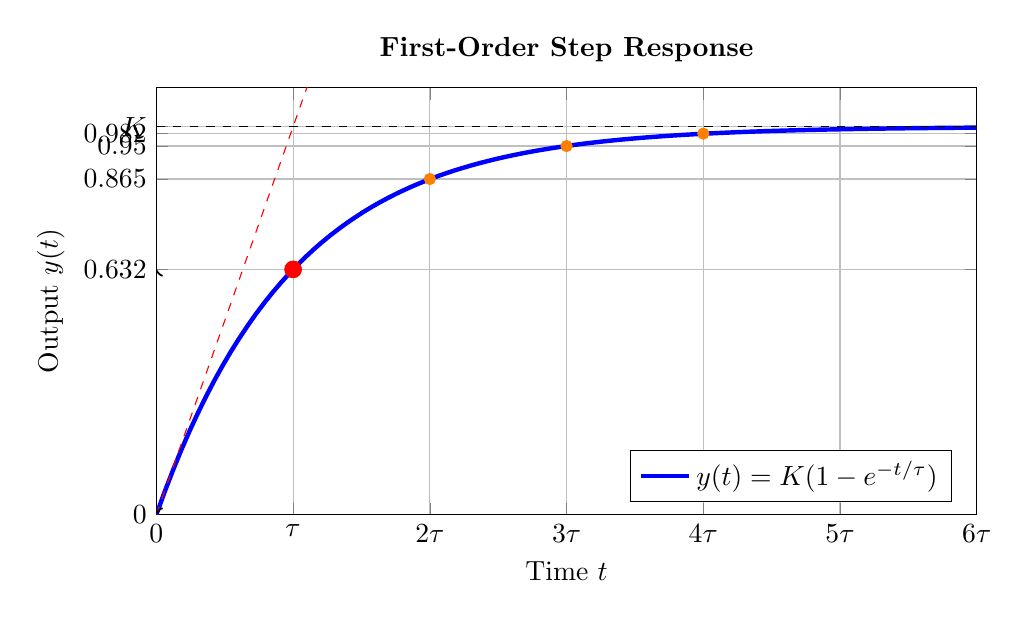
\begin{tikzpicture}
\begin{axis}[
    width=12cm, height=7cm,
    xlabel={Time $t$},
    ylabel={Output $y(t)$},
    xmin=0, xmax=6,
    ymin=0, ymax=1.1,
    xtick={0,1,2,3,4,5,6},
    xticklabels={0,$\tau$,$2\tau$,$3\tau$,$4\tau$,$5\tau$,$6\tau$},
    ytick={0,0.632,0.865,0.95,0.982,1},
    yticklabels={0,0.632,0.865,0.95,0.982,$K$},
    grid=major,
    legend pos=south east,
    title={\textbf{First-Order Step Response}}
]
    % Step response curve
    \addplot[blue, ultra thick, domain=0:6, samples=100] {1-exp(-x)};
    \addlegendentry{$y(t) = K(1-e^{-t/\tau})$}

    % Final value
    \addplot[black, dashed, domain=0:6] {1};

    % Time constant markers
    \addplot[only marks, mark=*, mark size=3pt, red] coordinates {(1,0.632)};
    \addplot[only marks, mark=*, mark size=2pt, orange] coordinates {(2,0.865)};
    \addplot[only marks, mark=*, mark size=2pt, orange] coordinates {(3,0.95)};
    \addplot[only marks, mark=*, mark size=2pt, orange] coordinates {(4,0.982)};

    % Tangent line at origin
    \addplot[red, dashed, domain=0:1.2] {x};

    % Annotation for time constant
    \draw[<->, thick] (axis cs:0,0.632) -- node[left] {$63.2\%$} (axis cs:0,0);

\end{axis}
\end{tikzpicture}
\caption{First-order step response showing the characteristic exponential approach to steady state. The tangent line at $t=0$ intersects the steady-state value at $t=\tau$.}
\label{fig:first_order_step}
\end{figure}

\subsubsection{Key Time-Domain Specifications}

\begin{keyconceptbox}[First-Order Response Characteristics]
The \textbf{time constant} has fundamental significance: at $t = \tau$, the output reaches $63.2\%$ of its final value, since $y(\tau) = K(1 - e^{-1}) = K(1 - 0.368) = 0.632K$.

The \textbf{settling time} (2\% criterion), defined as the time to reach and stay within 2\% of the final value, is approximately $t_s \approx 4\tau$ since $e^{-4} \approx 0.018 \approx 2\%$.

The \textbf{rise time} from 10\% to 90\% is given by $t_r = \tau(\ln 0.9 - \ln 0.1) = \tau \ln 9 \approx 2.2\tau$.

The \textbf{initial slope} of the response is $K/\tau$, and the tangent line at $t=0$ intersects $y=K$ at $t=\tau$.
\end{keyconceptbox}

%-----------------------------------------------------------------------------
\subsection{Second-Order Systems}
%-----------------------------------------------------------------------------

\begin{definition}[Standard Second-Order Transfer Function]
A second-order system in standard form is characterized by:
\begin{equation}
G(s) = \frac{\omega_n^2}{s^2 + 2\zeta\omega_n s + \omega_n^2}
\label{eq:second_order_tf}
\end{equation}
where $\omega_n > 0$ is the \textbf{natural frequency} (rad/s) and $\zeta \geq 0$ is the \textbf{damping ratio} (dimensionless).
\end{definition}

This transfer function has unity DC gain: $G(0) = 1$. For systems with gain $K \neq 1$, multiply the numerator by $K$.

\subsubsection{Physical Origin of Parameters}

Consider the canonical mass-spring-damper system:

\begin{center}
\begin{tikzpicture}[scale=1.0]
    % Wall
    \fill[pattern=north east lines] (-0.3,-0.5) rectangle (0,2);
    \draw[thick] (0,-0.5) -- (0,2);

    % Spring
    \draw[thick] (0,1.5) -- (0.5,1.5);
    \draw[thick,decorate,decoration={zigzag,segment length=4,amplitude=3}] (0.5,1.5) -- (2,1.5);
    \draw[thick] (2,1.5) -- (2.5,1.5);
    \node[above] at (1.25,1.7) {$k$};

    % Damper
    \draw[thick] (0,0.5) -- (0.5,0.5);
    \draw[thick] (0.5,0.2) rectangle (1.2,0.8);
    \draw[thick] (1.2,0.5) -- (1.5,0.5);
    \draw[thick] (1.5,0.3) -- (1.5,0.7);
    \draw[thick] (1.5,0.5) -- (2.5,0.5);
    \node[above] at (0.85,0.85) {$c$};

    % Mass
    \draw[thick,fill=gray!30] (2.5,0) rectangle (4,2);
    \node at (3.25,1) {$m$};

    % Force arrow
    \draw[->,ultra thick] (4,1) -- (5,1);
    \node[right] at (5,1) {$F(t)$};

    % Displacement
    \draw[<->] (3.25,-0.5) -- (4.5,-0.5);
    \node[below] at (3.875,-0.5) {$x(t)$};
\end{tikzpicture}
\end{center}

Newton's second law gives:
\begin{equation}
m\ddot{x} + c\dot{x} + kx = F(t)
\end{equation}

Taking the Laplace transform:
\begin{equation}
G(s) = \frac{X(s)}{F(s)} = \frac{1}{ms^2 + cs + k} = \frac{1/m}{s^2 + (c/m)s + k/m}
\end{equation}

Comparing with the standard form:
\begin{equation}
\boxed{\omega_n = \sqrt{\frac{k}{m}}, \qquad \zeta = \frac{c}{2\sqrt{km}} = \frac{c}{2m\omega_n}}
\label{eq:physical_params}
\end{equation}

The \textbf{natural frequency} $\omega_n$ is the frequency at which the undamped system would oscillate (when $c=0$). The \textbf{damping ratio} $\zeta$ compares the actual damping to the critical damping $c_{cr} = 2\sqrt{km}$.

\subsubsection{Characteristic Equation and Poles}

The characteristic equation is:
\begin{equation}
s^2 + 2\zeta\omega_n s + \omega_n^2 = 0
\end{equation}

Applying the quadratic formula:
\begin{equation}
\boxed{s_{1,2} = -\zeta\omega_n \pm \omega_n\sqrt{\zeta^2 - 1}}
\label{eq:poles}
\end{equation}

The nature of the roots depends critically on $\zeta$:

\begin{keyconceptbox}[Classification by Damping Ratio]
\textbf{Underdamped systems} ($0 < \zeta < 1$) have complex conjugate poles given by $s_{1,2} = -\zeta\omega_n \pm j\omega_n\sqrt{1-\zeta^2} = -\sigma \pm j\omega_d$, where $\sigma = \zeta\omega_n$ is the damping factor and $\omega_d = \omega_n\sqrt{1-\zeta^2}$ is the damped natural frequency.

\textbf{Critically damped systems} ($\zeta = 1$) have a repeated real pole at $s_{1,2} = -\omega_n$ (double pole).

\textbf{Overdamped systems} ($\zeta > 1$) have two distinct real poles at $s_{1,2} = -\zeta\omega_n \pm \omega_n\sqrt{\zeta^2 - 1}$. Both poles are negative (stable), with $s_1$ closer to the origin acting as the dominant pole.
\end{keyconceptbox}

\subsubsection{Step Response: Underdamped Case ($\zeta < 1$)}

For the underdamped case, the step response derivation yields:
\begin{equation}
\boxed{y(t) = 1 - \frac{e^{-\zeta\omega_n t}}{\sqrt{1-\zeta^2}}\sin\left(\omega_d t + \phi\right), \quad t \geq 0}
\label{eq:underdamped_step}
\end{equation}
where $\omega_d = \omega_n\sqrt{1-\zeta^2}$ and $\phi = \arctan\left(\sqrt{1-\zeta^2}/\zeta\right) = \arccos(\zeta)$.

An equivalent and often more useful form is:
\begin{equation}
y(t) = 1 - e^{-\zeta\omega_n t}\left(\cos\omega_d t + \frac{\zeta}{\sqrt{1-\zeta^2}}\sin\omega_d t\right)
\end{equation}

\subsubsection{Step Response: Critically Damped Case ($\zeta = 1$)}

When $\zeta = 1$, we have a repeated pole at $s = -\omega_n$:
\begin{equation}
\boxed{y(t) = 1 - e^{-\omega_n t}(1 + \omega_n t), \quad t \geq 0}
\label{eq:critical_step}
\end{equation}

This represents the fastest non-oscillatory response---any reduction in $\zeta$ causes overshoot, while any increase causes sluggishness.

\subsubsection{Step Response: Overdamped Case ($\zeta > 1$)}

For the overdamped case, define:
\begin{align}
s_1 &= -\zeta\omega_n + \omega_n\sqrt{\zeta^2-1} = -\omega_n(\zeta - \sqrt{\zeta^2-1}) \\
s_2 &= -\zeta\omega_n - \omega_n\sqrt{\zeta^2-1} = -\omega_n(\zeta + \sqrt{\zeta^2-1})
\end{align}

Note that $|s_2| > |s_1|$, so $s_1$ is the dominant (slower) pole. The step response is:
\begin{equation}
\boxed{y(t) = 1 - \frac{s_2}{s_2-s_1}e^{s_1 t} + \frac{s_1}{s_2-s_1}e^{s_2 t}, \quad t \geq 0}
\label{eq:overdamped_step}
\end{equation}

For large $\zeta$, $s_2 \gg s_1$ and the response is dominated by the slower mode.

\begin{figure}[H]
\centering
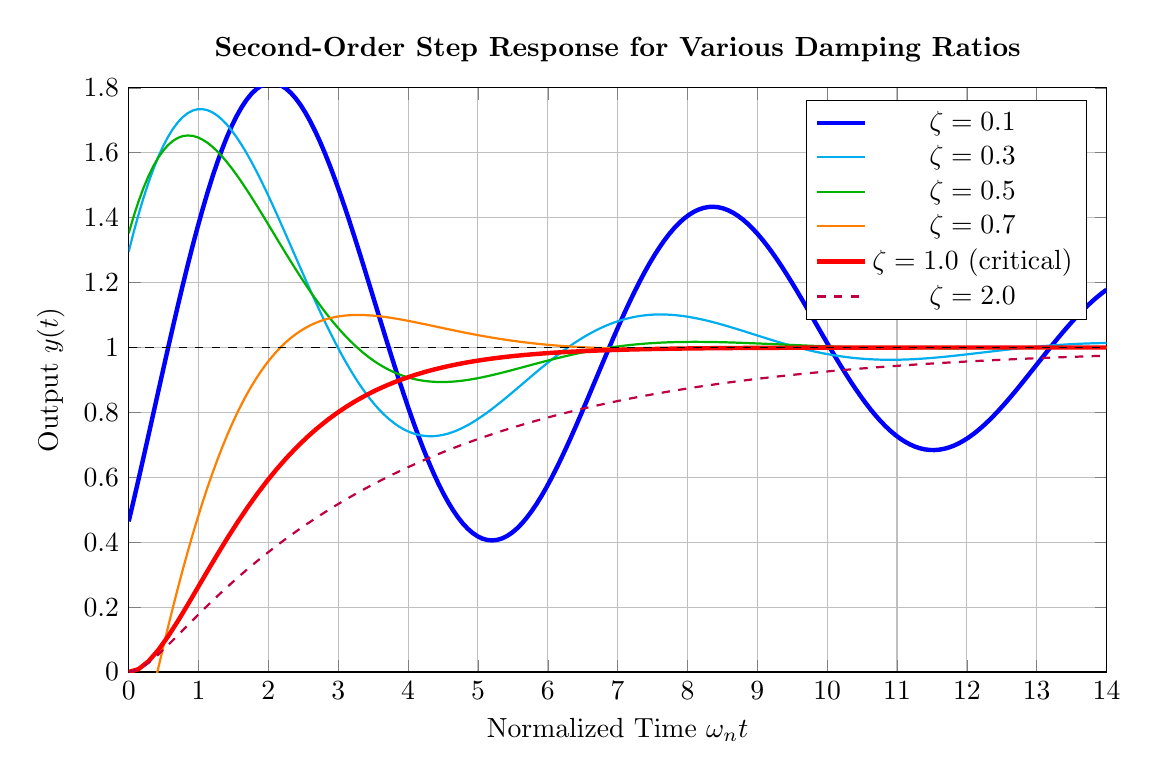
\begin{tikzpicture}
\begin{axis}[
    width=14cm, height=9cm,
    xlabel={Normalized Time $\omega_n t$},
    ylabel={Output $y(t)$},
    xmin=0, xmax=14,
    ymin=0, ymax=1.8,
    grid=major,
    legend style={at={(0.98,0.98)}, anchor=north east},
    title={\textbf{Second-Order Step Response for Various Damping Ratios}}
]
    % Underdamped: zeta = 0.1
    \addplot[blue, ultra thick, domain=0:14, samples=200]
        {1 - exp(-0.1*x)/sqrt(1-0.01)*sin(deg(sqrt(1-0.01)*x) + deg(acos(0.1)))};
    \addlegendentry{$\zeta = 0.1$}

    % Underdamped: zeta = 0.3
    \addplot[cyan, thick, domain=0:14, samples=200]
        {1 - exp(-0.3*x)/sqrt(1-0.09)*sin(deg(sqrt(1-0.09)*x) + deg(acos(0.3)))};
    \addlegendentry{$\zeta = 0.3$}

    % Underdamped: zeta = 0.5
    \addplot[green!70!black, thick, domain=0:14, samples=200]
        {1 - exp(-0.5*x)/sqrt(1-0.25)*sin(deg(sqrt(1-0.25)*x) + deg(acos(0.5)))};
    \addlegendentry{$\zeta = 0.5$}

    % Underdamped: zeta = 0.7
    \addplot[orange, thick, domain=0:14, samples=200]
        {1 - exp(-0.7*x)/sqrt(1-0.49)*sin(deg(sqrt(1-0.49)*x) + deg(acos(0.7)))};
    \addlegendentry{$\zeta = 0.7$}

    % Critical: zeta = 1.0
    \addplot[red, ultra thick, domain=0:14, samples=100]
        {1 - exp(-x)*(1 + x)};
    \addlegendentry{$\zeta = 1.0$ (critical)}

    % Overdamped: zeta = 2.0
    \addplot[purple, thick, dashed, domain=0:14, samples=100]
        {1 - (2+sqrt(3))/(2*sqrt(3))*exp(-(2-sqrt(3))*x) + (2-sqrt(3))/(2*sqrt(3))*exp(-(2+sqrt(3))*x)};
    \addlegendentry{$\zeta = 2.0$}

    % Final value line
    \addplot[black, dashed, domain=0:14] {1};

\end{axis}
\end{tikzpicture}
\caption{Step responses for second-order systems with various damping ratios. Underdamped responses ($\zeta < 1$) exhibit overshoot and oscillation. The critically damped response ($\zeta = 1$) is the fastest without overshoot. Overdamped responses ($\zeta > 1$) are sluggish.}
\label{fig:second_order_step}
\end{figure}

\subsubsection{Time-Domain Specifications for Underdamped Systems}

For underdamped second-order systems, several key specifications characterize the transient response:

\begin{keyconceptbox}[Second-Order Transient Response Specifications]
\textbf{Percent Overshoot (PO):}
\begin{equation}
\boxed{PO = e^{-\pi\zeta/\sqrt{1-\zeta^2}} \times 100\%}
\label{eq:overshoot}
\end{equation}
Depends only on $\zeta$, not on $\omega_n$.

\textbf{Peak Time} (time to first peak):
\begin{equation}
\boxed{t_p = \frac{\pi}{\omega_d} = \frac{\pi}{\omega_n\sqrt{1-\zeta^2}}}
\label{eq:peak_time}
\end{equation}

\textbf{Rise Time} (0\% to 100\%, approximate):
\begin{equation}
\boxed{t_r \approx \frac{1.8}{\omega_n} \quad \text{for } 0.3 < \zeta < 0.8}
\label{eq:rise_time}
\end{equation}

\textbf{Settling Time} (2\% criterion):
\begin{equation}
\boxed{t_s \approx \frac{4}{\zeta\omega_n} = \frac{4}{\sigma}}
\label{eq:settling_time}
\end{equation}
\end{keyconceptbox}

\begin{table}[H]
\centering
\caption{Percent Overshoot vs. Damping Ratio}
\label{tab:overshoot}
\begin{tabular}{cc|cc|cc}
\toprule
$\zeta$ & PO (\%) & $\zeta$ & PO (\%) & $\zeta$ & PO (\%) \\
\midrule
0.1 & 72.9 & 0.4 & 25.4 & 0.7 & 4.6 \\
0.2 & 52.7 & 0.5 & 16.3 & 0.8 & 1.5 \\
0.3 & 37.2 & 0.6 & 9.5 & 0.9 & 0.2 \\
\bottomrule
\end{tabular}
\end{table}

%-----------------------------------------------------------------------------
\subsection{Pole Locations and Response Characteristics}
%-----------------------------------------------------------------------------

The location of poles in the complex $s$-plane provides immediate insight into system behavior. This geometric interpretation is one of the most powerful tools in control system analysis.

\begin{figure}[H]
\centering
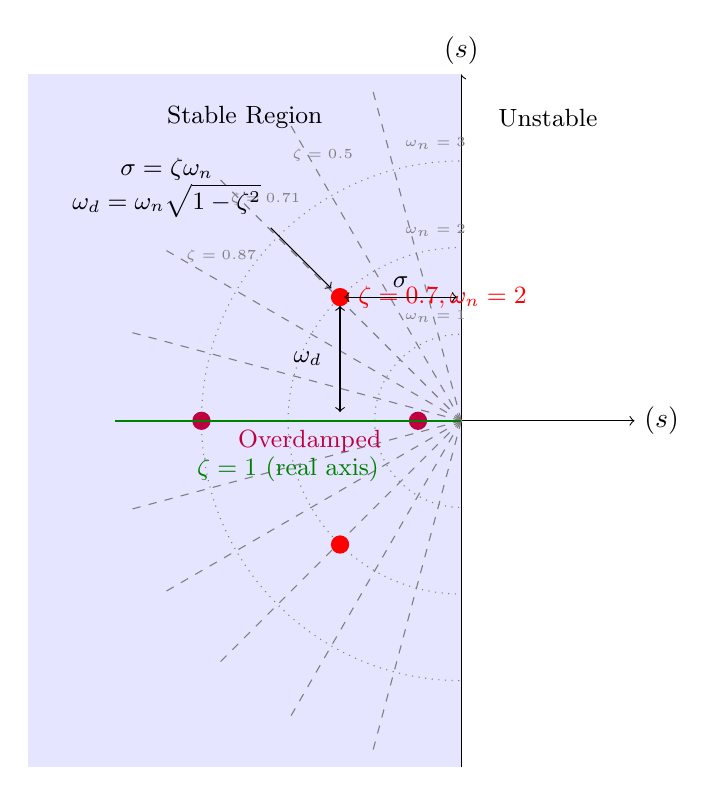
\begin{tikzpicture}[scale=1.1]
    % Axes
    \draw[->] (-5,0) -- (2,0) node[right] {$\real(s)$};
    \draw[->] (0,-4) -- (0,4) node[above] {$\imag(s)$};

    % Stable region shading
    \fill[blue!10] (-5,-4) rectangle (0,4);
    \node at (-2.5,3.5) {\small Stable Region};

    % Unstable region label
    \node at (1,3.5) {\small Unstable};

    % Constant zeta lines (radial lines from origin)
    \foreach \angle/\zeta in {15/0.97, 30/0.87, 45/0.71, 60/0.5, 75/0.26} {
        \draw[gray, dashed] (0,0) -- ({-4*cos(\angle)},{4*sin(\angle)});
        \draw[gray, dashed] (0,0) -- ({-4*cos(\angle)},{-4*sin(\angle)});
    }
    \node[gray] at ({-3.2*cos(30)},{3.2*sin(30)+0.3}) {\tiny $\zeta=0.87$};
    \node[gray] at ({-3.2*cos(45)},{3.2*sin(45)+0.3}) {\tiny $\zeta=0.71$};
    \node[gray] at ({-3.2*cos(60)},{3.2*sin(60)+0.3}) {\tiny $\zeta=0.5$};

    % Constant omega_n circles (semicircles in LHP)
    \foreach \r in {1,2,3} {
        \draw[gray, dotted] (0,0) ++(180:\r) arc (180:270:\r);
        \draw[gray, dotted] (0,0) ++(180:\r) arc (180:90:\r);
    }
    \node[gray] at (-0.3,1.2) {\tiny $\omega_n=1$};
    \node[gray] at (-0.3,2.2) {\tiny $\omega_n=2$};
    \node[gray] at (-0.3,3.2) {\tiny $\omega_n=3$};

    % Example poles - underdamped
    \fill[red] ({-0.7*2},{sqrt(1-0.49)*2}) circle (3pt);
    \fill[red] ({-0.7*2},{-sqrt(1-0.49)*2}) circle (3pt);
    \node[red, right] at ({-0.7*2+0.1},{sqrt(1-0.49)*2}) {\small $\zeta=0.7, \omega_n=2$};

    % Example poles - overdamped
    \fill[purple] (-0.5,0) circle (3pt);
    \fill[purple] (-3,0) circle (3pt);
    \node[purple, below] at (-1.75,0) {\small Overdamped};

    % Critical damping line
    \draw[green!50!black, thick] (-4,0) -- (0,0);
    \node[green!50!black, below] at (-2,-0.3) {\small $\zeta=1$ (real axis)};

    % Annotations
    \draw[<-] ({-0.7*2-0.1},{sqrt(1-0.49)*2+0.1}) -- ({-0.7*2-0.8},{sqrt(1-0.49)*2+0.8})
        node[above left, align=center] {\small $\sigma = \zeta\omega_n$ \\ \small $\omega_d = \omega_n\sqrt{1-\zeta^2}$};

    % Sigma and omega_d labels
    \draw[<->] ({-0.7*2},0.1) -- ({-0.7*2},{sqrt(1-0.49)*2-0.1});
    \node[left] at ({-0.7*2-0.1},{sqrt(1-0.49)*2/2}) {\small $\omega_d$};
    \draw[<->] (-0.05,{sqrt(1-0.49)*2}) -- ({-0.7*2+0.05},{sqrt(1-0.49)*2});
    \node[above] at ({-0.7},{sqrt(1-0.49)*2}) {\small $\sigma$};

\end{tikzpicture}
\caption{The $s$-plane showing regions of constant damping ratio (radial lines from origin) and constant natural frequency (semicircles). Poles in the left half-plane are stable; poles on the real axis correspond to $\zeta \geq 1$.}
\label{fig:s_plane}
\end{figure}

Key observations from the $s$-plane representation connect pole geometry to dynamic behavior. The \textbf{horizontal distance from the imaginary axis}, $\sigma = \zeta\omega_n$, determines the exponential decay rate; larger $\sigma$ means faster settling. The \textbf{vertical distance from the real axis}, $\omega_d = \omega_n\sqrt{1-\zeta^2}$, determines the oscillation frequency, with larger $\omega_d$ producing faster oscillation. The \textbf{distance from the origin}, $\omega_n = \sqrt{\sigma^2 + \omega_d^2}$, equals the natural frequency. Finally, the \textbf{angle from the negative real axis}, $\theta = \arccos\zeta$, is directly related to the damping ratio.

\begin{figure}[H]
\centering
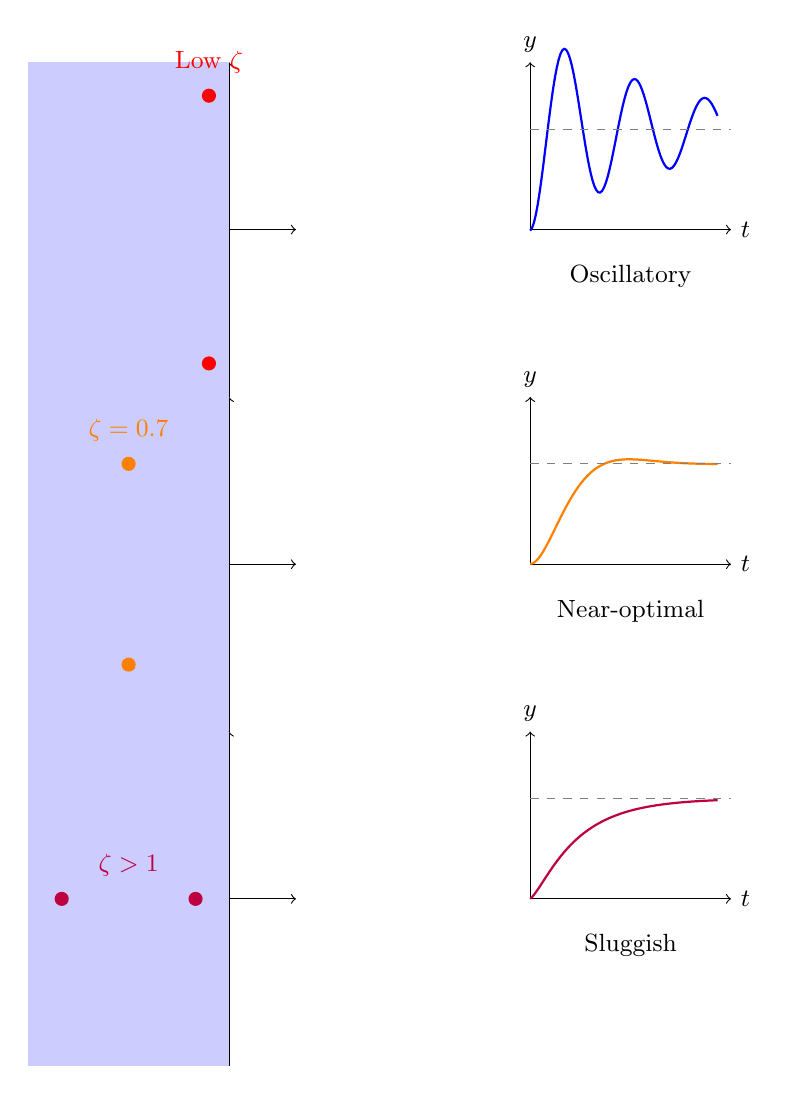
\begin{tikzpicture}[scale=0.85]
    % Main s-plane
    \begin{scope}[shift={(0,0)}]
        \draw[->] (-3,0) -- (1,0) node[right] {$\real$};
        \draw[->] (0,-2.5) -- (0,2.5) node[above] {$\imag$};
        \fill[blue!20] (-3,-2.5) rectangle (0,2.5);

        % Pole near imaginary axis (lightly damped)
        \fill[red] (-0.3,2) circle (3pt);
        \fill[red] (-0.3,-2) circle (3pt);
        \node[red] at (-0.3,2.5) {\small Low $\zeta$};
    \end{scope}

    % Response plot 1
    \begin{scope}[shift={(4.5,0)}]
        \draw[->] (0,0) -- (3,0) node[right] {\small $t$};
        \draw[->] (0,0) -- (0,2.5) node[above] {\small $y$};
        \draw[blue, thick, domain=0:2.8, samples=100] plot (\x, {1.5*(1-exp(-0.15*\x*3)*cos(deg(2*\x*3))/0.99)});
        \draw[gray, dashed] (0,1.5) -- (3,1.5);
        \node at (1.5,-0.7) {\small Oscillatory};
    \end{scope}

    % Second s-plane
    \begin{scope}[shift={(0,-5)}]
        \draw[->] (-3,0) -- (1,0) node[right] {$\real$};
        \draw[->] (0,-2.5) -- (0,2.5) node[above] {$\imag$};
        \fill[blue!20] (-3,-2.5) rectangle (0,2.5);

        % Poles at 45 degrees
        \fill[orange] (-1.5,1.5) circle (3pt);
        \fill[orange] (-1.5,-1.5) circle (3pt);
        \node[orange] at (-1.5,2) {\small $\zeta=0.7$};
    \end{scope}

    % Response plot 2
    \begin{scope}[shift={(4.5,-5)}]
        \draw[->] (0,0) -- (3,0) node[right] {\small $t$};
        \draw[->] (0,0) -- (0,2.5) node[above] {\small $y$};
        \draw[orange, thick, domain=0:2.8, samples=100] plot (\x, {1.5*(1-exp(-0.7*\x*3)/0.71*sin(deg(0.71*\x*3)+45))});
        \draw[gray, dashed] (0,1.5) -- (3,1.5);
        \node at (1.5,-0.7) {\small Near-optimal};
    \end{scope}

    % Third s-plane
    \begin{scope}[shift={(0,-10)}]
        \draw[->] (-3,0) -- (1,0) node[right] {$\real$};
        \draw[->] (0,-2.5) -- (0,2.5) node[above] {$\imag$};
        \fill[blue!20] (-3,-2.5) rectangle (0,2.5);

        % Poles on real axis (overdamped)
        \fill[purple] (-0.5,0) circle (3pt);
        \fill[purple] (-2.5,0) circle (3pt);
        \node[purple] at (-1.5,0.5) {\small $\zeta>1$};
    \end{scope}

    % Response plot 3
    \begin{scope}[shift={(4.5,-10)}]
        \draw[->] (0,0) -- (3,0) node[right] {\small $t$};
        \draw[->] (0,0) -- (0,2.5) node[above] {\small $y$};
        \draw[purple, thick, domain=0:2.8, samples=100] plot (\x, {1.5*(1-1.15*exp(-0.5*\x*3)+0.15*exp(-2.5*\x*3))});
        \draw[gray, dashed] (0,1.5) -- (3,1.5);
        \node at (1.5,-0.7) {\small Sluggish};
    \end{scope}

\end{tikzpicture}
\caption{Relationship between pole locations and step response characteristics. Top: lightly damped (poles near imaginary axis). Middle: well-damped (poles at $45°$). Bottom: overdamped (poles on real axis).}
\label{fig:poles_responses}
\end{figure}

%=============================================================================
\section{Laboratory Experiment: Variable Damping Mass-Spring System}
%=============================================================================

This section describes a hands-on experiment to build and characterize a second-order mechanical system with adjustable damping. Students will observe the transition from underdamped to critically damped to overdamped response and extract system parameters from measured data.

\begin{experimentbox}[Learning Objectives]
Upon completion of this experiment, students will be able to construct a physical mass-spring-damper system with variable damping, measure step response using digital instrumentation, extract $\zeta$ and $\omega_n$ from experimental data, and correlate physical damping changes with observed response characteristics.
\end{experimentbox}

%-----------------------------------------------------------------------------
\subsection{Apparatus Design and Construction}
%-----------------------------------------------------------------------------

\subsubsection{Frame and Mass Assembly}

The experimental apparatus consists of a vertical mass-spring system with adjustable viscous damping. The frame can be constructed from 3D-printed components, aluminum extrusion, or wooden dowels.

\textbf{Bill of Materials:}

\begin{center}
\begin{tabular}{lp{8cm}}
\toprule
\textbf{Component} & \textbf{Specification} \\
\midrule
Vertical guide rail & Aluminum or 3D-printed, 300mm length \\
Mass carrier & 3D-printed or machined block, approximately 100g base mass \\
Additional masses & Washers, nuts, or calibrated weights (50g, 100g, 200g) \\
Linear bearings & Low-friction sleeve for vertical motion \\
Mounting base & Stable platform to prevent vibration \\
\bottomrule
\end{tabular}
\end{center}

\subsubsection{Spring Element}

For accessible experimentation, rubber bands provide variable spring constants. Use consistent rubber bands (size \#64 or similar) for reproducibility. Parallel bands increase $k$ while a series arrangement decreases $k$. Alternatively, extension springs from a hardware store with known spring constants can be used for more precise measurements.

Characterize the spring constant by hanging known masses and measuring displacement:
\begin{equation}
k = \frac{mg}{\Delta x}
\end{equation}

\subsubsection{Variable Damping Mechanism}

Three options for adjustable damping are presented:

\begin{center}
\begin{tabular}{lp{10cm}}
\toprule
\textbf{Option} & \textbf{Description and Adjustment Method} \\
\midrule
\textbf{A: Water Dashpot} & A cylinder partially filled with water contains a plunger attached to the moving mass with orifices of various sizes. Damping is varied by changing orifice size or water viscosity (add glycerin). \\
\addlinespace
\textbf{B: Eddy Current Damper} & An aluminum or copper plate attached to the moving mass passes near permanent magnets. Damping is adjusted by varying magnet proximity. This option provides smooth, velocity-proportional damping. \\
\addlinespace
\textbf{C: Friction Pad} & A felt or foam pad is pressed against the guide rail with adjustable normal force via a thumbscrew. Note: this provides approximately velocity-independent Coulomb friction rather than ideal viscous damping. \\
\bottomrule
\end{tabular}
\end{center}

\subsubsection{Instrumentation}

\textbf{Distance Measurement:}

\begin{center}
\begin{tabular}{lll}
\toprule
\textbf{Sensor} & \textbf{Range} & \textbf{Resolution} \\
\midrule
Ultrasonic (HC-SR04) & 2cm--400cm & $\sim$3mm \\
Time-of-flight (VL53L0X) & 3cm--200cm & $\sim$1mm \\
Infrared (Sharp GP2Y0A21) & 10cm--80cm & $\sim$2mm \\
\bottomrule
\end{tabular}
\end{center}

\textbf{Data Acquisition:}

Data acquisition requires an Arduino Uno or similar microcontroller operating at a minimum sampling rate of 50~Hz, though 100+~Hz is preferable for capturing fast dynamics. Data can be logged to a serial monitor for real-time viewing or to an SD card for later analysis.

\textbf{Arduino Code Framework:}
\begin{verbatim}
// Second-order system measurement
const int trigPin = 9;
const int echoPin = 10;
unsigned long startTime;

void setup() {
  Serial.begin(115200);
  pinMode(trigPin, OUTPUT);
  pinMode(echoPin, INPUT);
  startTime = millis();
}

void loop() {
  float distance = measureDistance();
  unsigned long elapsed = millis() - startTime;
  Serial.print(elapsed);
  Serial.print(",");
  Serial.println(distance);
  delay(10);  // 100 Hz sampling
}

float measureDistance() {
  digitalWrite(trigPin, LOW);
  delayMicroseconds(2);
  digitalWrite(trigPin, HIGH);
  delayMicroseconds(10);
  digitalWrite(trigPin, LOW);
  long duration = pulseIn(echoPin, HIGH);
  return duration * 0.034 / 2;  // cm
}
\end{verbatim}

%-----------------------------------------------------------------------------
\subsection{Experimental Procedure}
%-----------------------------------------------------------------------------

\subsubsection{System Characterization}

System characterization proceeds in four stages. First, \textbf{measure the mass} by weighing the total moving mass $m$ including the carrier, sensor mount, and any added weights. Second, \textbf{measure the spring constant} with the damping mechanism removed; displace the mass by measured amounts, apply several known forces, and calculate $k$ from the slope of force vs.\ displacement. Third, \textbf{predict the natural frequency} by calculating $\omega_n = \sqrt{k/m}$ and $f_n = \omega_n/(2\pi)$. Finally, \textbf{verify the undamped frequency} by applying a step input with minimal damping and measuring the oscillation period $T$, then compare $f_{measured} = 1/T$ with the prediction.

\subsubsection{Step Response Measurement}

To measure the step response, position the mass at a displaced equilibrium (e.g., compress the spring by 2--3~cm), then start data acquisition. Release the mass smoothly, taking care not to impart any initial velocity. Record position vs.\ time for at least 5 natural periods or until the system settles. Repeat the measurement 3--5 times for statistical confidence.

\subsubsection{Damping Variation Study}

Perform the step response measurement for at least four damping levels: minimal damping (underdamped with high oscillation), moderate damping (underdamped with visible overshoot), high damping (near critical with minimal overshoot), and maximum damping (overdamped with no oscillation).

%-----------------------------------------------------------------------------
\subsection{Data Analysis and Parameter Extraction}
%-----------------------------------------------------------------------------

\subsubsection{Extracting Parameters from Underdamped Response}

Given a measured underdamped step response, extract $\zeta$ and $\omega_n$ using the following methods:

\textbf{Method 1: Logarithmic Decrement}

Measure successive peak amplitudes $x_1, x_2, x_3, \ldots$ above the final value. The logarithmic decrement is:
\begin{equation}
\delta = \ln\left(\frac{x_n}{x_{n+1}}\right)
\end{equation}

The damping ratio is:
\begin{equation}
\zeta = \frac{\delta}{\sqrt{4\pi^2 + \delta^2}}
\end{equation}

For small damping, $\zeta \approx \delta/(2\pi)$.

\textbf{Method 2: Percent Overshoot}

Measure the first peak value $y_{max}$ and final value $y_{ss}$:
\begin{equation}
PO = \frac{y_{max} - y_{ss}}{y_{ss}} \times 100\%
\end{equation}

Solve for $\zeta$:
\begin{equation}
\zeta = \frac{-\ln(PO/100)}{\sqrt{\pi^2 + \ln^2(PO/100)}}
\end{equation}

\textbf{Method 3: Damped Period Measurement}

Measure the period of oscillation $T_d$ between successive peaks:
\begin{equation}
\omega_d = \frac{2\pi}{T_d}
\end{equation}

With $\zeta$ known from overshoot:
\begin{equation}
\omega_n = \frac{\omega_d}{\sqrt{1-\zeta^2}}
\end{equation}

\subsubsection{Extracting Parameters from Overdamped Response}

For overdamped systems, fitting the response to a sum of two exponentials is required:
\begin{equation}
y(t) = y_{ss}\left(1 - A_1 e^{-t/\tau_1} - A_2 e^{-t/\tau_2}\right)
\end{equation}

Use nonlinear curve fitting (MATLAB's \texttt{fit} or Python's \texttt{scipy.optimize.curve\_fit}) to extract $\tau_1$ and $\tau_2$. The poles are $s_1 = -1/\tau_1$ and $s_2 = -1/\tau_2$.

\subsubsection{Sample Data Analysis}

\begin{table}[H]
\centering
\caption{Sample Experimental Results}
\label{tab:sample_results}
\begin{tabular}{lccccc}
\toprule
\textbf{Damping Setting} & \textbf{PO (\%)} & $\boldsymbol{\zeta}$ & $\boldsymbol{T_d}$ (s) & $\boldsymbol{\omega_n}$ (rad/s) & \textbf{Behavior} \\
\midrule
Minimal & 52 & 0.21 & 0.45 & 14.3 & Underdamped \\
Low & 25 & 0.40 & 0.48 & 14.3 & Underdamped \\
Medium & 5 & 0.69 & 0.55 & 15.8 & Underdamped \\
High & 0 & $>1$ & --- & 14.1 & Overdamped \\
\bottomrule
\end{tabular}
\end{table}

\subsection{Discussion Questions}

Consider the following questions when analyzing your experimental results. Why does $\omega_n$ remain approximately constant across damping settings? What practical limitations prevent achieving exactly $\zeta = 1$ (critical damping)? How does the friction-based damper differ from ideal viscous damping, and what effect does this have on the response shape? If you wanted to double the natural frequency without changing the damping ratio, what physical parameters would you modify? Finally, compare your measured settling times with the theoretical prediction $t_s = 4/(\zeta\omega_n)$ and identify sources of error that might explain any discrepancies.

%=============================================================================
\section{Worked Examples}
%=============================================================================

This section presents detailed solutions to representative problems involving first and second order systems. Each example emphasizes a specific concept or technique.

%-----------------------------------------------------------------------------
\begin{example}[Time Constant from RC Circuit Values]
\label{ex:rc_circuit}
An RC low-pass filter has $R = 10\,\text{k}\Omega$ and $C = 47\,\mu\text{F}$. Find:
\begin{enumerate}[label=(\alph*)]
    \item The time constant $\tau$
    \item The transfer function
    \item The settling time (2\% criterion)
    \item The output voltage 0.5 seconds after applying a 5V step input
\end{enumerate}
\end{example}

\textbf{Solution:}

\textbf{(a) Time Constant:}
\begin{equation}
\tau = RC = (10 \times 10^3\,\Omega)(47 \times 10^{-6}\,\text{F}) = 0.47\,\text{s}
\end{equation}

\textbf{(b) Transfer Function:}
The standard first-order form is:
\begin{equation}
G(s) = \frac{1}{\tau s + 1} = \frac{1}{0.47s + 1}
\end{equation}

Or in terms of the pole location:
\begin{equation}
G(s) = \frac{2.13}{s + 2.13}
\end{equation}

The single pole is at $s = -1/\tau = -2.13\,\text{rad/s}$.

\textbf{(c) Settling Time:}
\begin{equation}
t_s = 4\tau = 4(0.47) = 1.88\,\text{s}
\end{equation}

\textbf{(d) Output Voltage at $t = 0.5\,\text{s}$:}

For a 5V step input:
\begin{equation}
v_{out}(t) = 5\left(1 - e^{-t/\tau}\right) = 5\left(1 - e^{-0.5/0.47}\right)
\end{equation}
\begin{equation}
v_{out}(0.5) = 5\left(1 - e^{-1.064}\right) = 5(1 - 0.345) = 5(0.655) = \boxed{3.28\,\text{V}}
\end{equation}

This represents 65.5\% of the final value, consistent with being just past one time constant.

\hfill$\square$

%-----------------------------------------------------------------------------
\begin{example}[Finding $\zeta$ and $\omega_n$ from Transfer Function]
\label{ex:tf_params}
Given the transfer function:
\begin{equation}
G(s) = \frac{50}{s^2 + 6s + 25}
\end{equation}
Determine $\omega_n$, $\zeta$, the pole locations, and characterize the expected step response.
\end{example}

\textbf{Solution:}

Compare with the standard form $G(s) = K\omega_n^2/(s^2 + 2\zeta\omega_n s + \omega_n^2)$:
\begin{equation}
s^2 + 2\zeta\omega_n s + \omega_n^2 = s^2 + 6s + 25
\end{equation}

Therefore:
\begin{align}
\omega_n^2 &= 25 \implies \boxed{\omega_n = 5\,\text{rad/s}} \\
2\zeta\omega_n &= 6 \implies \zeta = \frac{6}{2(5)} = \boxed{0.6}
\end{align}

The DC gain is $K = 50/25 = 2$.

\textbf{Pole Locations:}
\begin{align}
s_{1,2} &= -\zeta\omega_n \pm j\omega_n\sqrt{1-\zeta^2} \\
&= -0.6(5) \pm j(5)\sqrt{1-0.36} \\
&= -3 \pm j(5)(0.8) \\
&= \boxed{-3 \pm j4}
\end{align}

\textbf{Response Characteristics:}

Since $\zeta = 0.6 < 1$, the system is \textbf{underdamped}.

Percent overshoot:
\begin{equation}
PO = e^{-\pi(0.6)/\sqrt{1-0.36}} \times 100\% = e^{-\pi(0.6)/0.8} \times 100\% = e^{-2.356} \times 100\% \approx \boxed{9.5\%}
\end{equation}

Damped frequency:
\begin{equation}
\omega_d = \omega_n\sqrt{1-\zeta^2} = 5(0.8) = 4\,\text{rad/s}
\end{equation}

Peak time:
\begin{equation}
t_p = \frac{\pi}{\omega_d} = \frac{\pi}{4} \approx 0.785\,\text{s}
\end{equation}

Settling time:
\begin{equation}
t_s = \frac{4}{\zeta\omega_n} = \frac{4}{0.6 \times 5} = \frac{4}{3} \approx 1.33\,\text{s}
\end{equation}

\hfill$\square$

%-----------------------------------------------------------------------------
\begin{example}[Calculating Overshoot and Settling Time]
\label{ex:specs}
A second-order system has natural frequency $\omega_n = 10\,\text{rad/s}$ and damping ratio $\zeta = 0.4$. Calculate:
\begin{enumerate}[label=(\alph*)]
    \item Percent overshoot
    \item Peak time
    \item Settling time (2\% criterion)
    \item Rise time (approximate)
\end{enumerate}
\end{example}

\textbf{Solution:}

\textbf{(a) Percent Overshoot:}
\begin{equation}
PO = \exp\left(\frac{-\pi\zeta}{\sqrt{1-\zeta^2}}\right) \times 100\%
\end{equation}
\begin{equation}
PO = \exp\left(\frac{-\pi(0.4)}{\sqrt{1-0.16}}\right) \times 100\% = \exp\left(\frac{-1.257}{0.917}\right) \times 100\%
\end{equation}
\begin{equation}
PO = e^{-1.371} \times 100\% = 0.254 \times 100\% = \boxed{25.4\%}
\end{equation}

\textbf{(b) Peak Time:}

First, calculate the damped natural frequency:
\begin{equation}
\omega_d = \omega_n\sqrt{1-\zeta^2} = 10\sqrt{1-0.16} = 10(0.917) = 9.17\,\text{rad/s}
\end{equation}

Then:
\begin{equation}
t_p = \frac{\pi}{\omega_d} = \frac{\pi}{9.17} = \boxed{0.343\,\text{s}}
\end{equation}

\textbf{(c) Settling Time:}
\begin{equation}
t_s = \frac{4}{\zeta\omega_n} = \frac{4}{0.4 \times 10} = \frac{4}{4} = \boxed{1.0\,\text{s}}
\end{equation}

\textbf{(d) Rise Time (approximate formula for $0.3 < \zeta < 0.8$):}
\begin{equation}
t_r \approx \frac{1.8}{\omega_n} = \frac{1.8}{10} = \boxed{0.18\,\text{s}}
\end{equation}

A more accurate empirical formula is:
\begin{equation}
t_r \approx \frac{1 + 1.1\zeta + 1.4\zeta^2}{\omega_n} = \frac{1 + 0.44 + 0.224}{10} = \frac{1.664}{10} = 0.166\,\text{s}
\end{equation}

\hfill$\square$

%-----------------------------------------------------------------------------
\begin{example}[Pole Locations from Response Requirements]
\label{ex:pole_placement}
A control system must meet the following specifications: settling time $t_s \leq 2\,\text{s}$ and percent overshoot $PO \leq 10\%$. Determine the required region in the $s$-plane for the dominant poles.
\end{example}

\textbf{Solution:}

\textbf{Settling Time Constraint:}

The settling time constraint $t_s \leq 2\,\text{s}$ requires:
\begin{equation}
\frac{4}{\sigma} \leq 2 \implies \sigma \geq 2
\end{equation}

where $\sigma = \zeta\omega_n$ is the real part of the poles. This defines a vertical line at $\real(s) = -2$; poles must lie to the \textit{left} of this line.

\textbf{Overshoot Constraint:}

The overshoot constraint $PO \leq 10\%$ requires:
\begin{equation}
\exp\left(\frac{-\pi\zeta}{\sqrt{1-\zeta^2}}\right) \leq 0.10
\end{equation}

Taking the natural logarithm:
\begin{equation}
\frac{-\pi\zeta}{\sqrt{1-\zeta^2}} \leq \ln(0.10) = -2.303
\end{equation}

\begin{equation}
\frac{\pi\zeta}{\sqrt{1-\zeta^2}} \geq 2.303
\end{equation}

Squaring both sides:
\begin{equation}
\frac{\pi^2\zeta^2}{1-\zeta^2} \geq 5.304
\end{equation}

\begin{equation}
\pi^2\zeta^2 \geq 5.304 - 5.304\zeta^2
\end{equation}

\begin{equation}
\zeta^2(\pi^2 + 5.304) \geq 5.304
\end{equation}

\begin{equation}
\zeta^2 \geq \frac{5.304}{9.87 + 5.304} = \frac{5.304}{15.17} = 0.350
\end{equation}

\begin{equation}
\zeta \geq 0.591
\end{equation}

Since $\cos\theta = \zeta$, this corresponds to $\theta \leq \arccos(0.591) = 53.7°$ from the negative real axis.

\textbf{Combined Region:}

\begin{center}
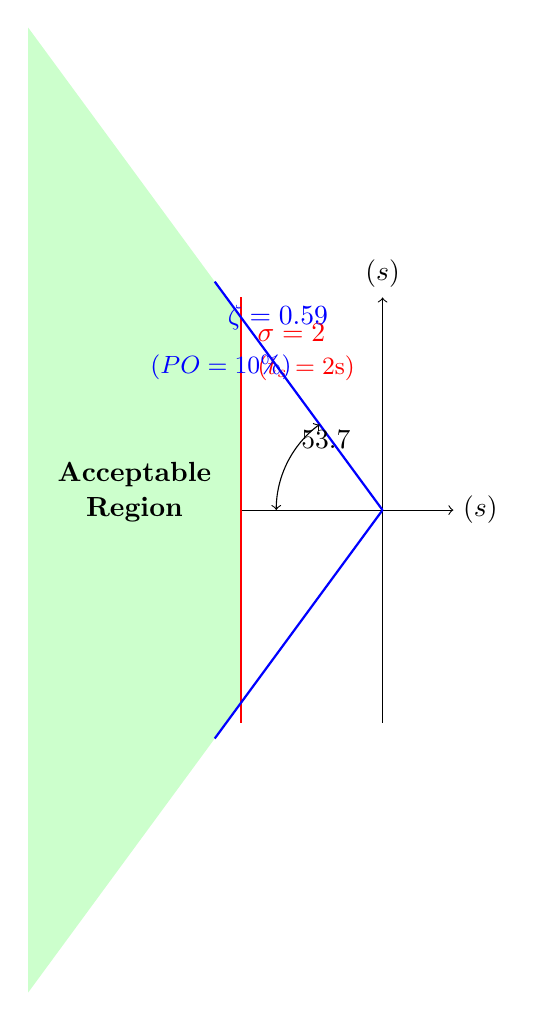
\begin{tikzpicture}[scale=0.9]
    % Axes
    \draw[->] (-5,0) -- (1,0) node[right] {$\real(s)$};
    \draw[->] (0,-3) -- (0,3) node[above] {$\imag(s)$};

    % Acceptable region (shaded)
    \fill[green!20] (-5,0) -- (-2,0) -- (-2,{2*tan(53.7)}) -- (-5,{5*tan(53.7)}) -- cycle;
    \fill[green!20] (-5,0) -- (-2,0) -- (-2,{-2*tan(53.7)}) -- (-5,{-5*tan(53.7)}) -- cycle;

    % Settling time line
    \draw[red, thick] (-2,-3) -- (-2,3);
    \node[red, right] at (-1.9,2.5) {$\sigma = 2$};
    \node[red, right] at (-1.9,2) {\small ($t_s = 2$s)};

    % Damping ratio lines
    \draw[blue, thick] (0,0) -- ({-4*cos(53.7)},{4*sin(53.7)});
    \draw[blue, thick] (0,0) -- ({-4*cos(53.7)},{-4*sin(53.7)});
    \node[blue] at ({-3*cos(53.7)+0.3},{3*sin(53.7)+0.3}) {$\zeta = 0.59$};
    \node[blue] at ({-2.5*cos(53.7)-0.8},{2.5*sin(53.7)}) {\small ($PO = 10\%$)};

    % Angle annotation
    \draw[<->] (-1.5,0) arc (180:126.3:1.5);
    \node at (-0.8,1) {$53.7°$};

    % Label acceptable region
    \node at (-3.5,0.5) {\textbf{Acceptable}};
    \node at (-3.5,0) {\textbf{Region}};

\end{tikzpicture}
\end{center}

The dominant poles must be placed in the shaded region: to the left of $\real(s) = -2$ and within $\pm 53.7°$ of the negative real axis.

One acceptable pole pair would be:
\begin{equation}
s = -3 \pm j2.5 \quad (\sigma = 3, \omega_d = 2.5, \zeta = 0.77, \omega_n = 3.91)
\end{equation}

Verification: $t_s = 4/3 = 1.33\,\text{s} < 2\,\text{s}$ \checkmark, and $PO = 2.6\% < 10\%$ \checkmark.

\hfill$\square$

%-----------------------------------------------------------------------------
\begin{example}[System Identification from Step Response]
\label{ex:sysid}
The following step response data was measured from an unknown second-order system: the final (steady-state) value is $y_{ss} = 2.0$, the first peak value is $y_{max} = 2.52$ occurring at $t_p = 0.25\,\text{s}$, and the second peak value is $y_2 = 2.20$ at $t = 0.5\,\text{s}$. Determine the transfer function of the system.
\end{example}

\textbf{Solution:}

\textbf{Step 1: Calculate Percent Overshoot}
\begin{equation}
PO = \frac{y_{max} - y_{ss}}{y_{ss}} \times 100\% = \frac{2.52 - 2.0}{2.0} \times 100\% = 26\%
\end{equation}

\textbf{Step 2: Find Damping Ratio from Overshoot}
\begin{equation}
\zeta = \frac{-\ln(PO/100)}{\sqrt{\pi^2 + \ln^2(PO/100)}} = \frac{-\ln(0.26)}{\sqrt{\pi^2 + \ln^2(0.26)}}
\end{equation}
\begin{equation}
\zeta = \frac{1.347}{\sqrt{9.87 + 1.814}} = \frac{1.347}{\sqrt{11.68}} = \frac{1.347}{3.42} = 0.394
\end{equation}

\textbf{Step 3: Verify Using Logarithmic Decrement}

The ratio of successive overshoots:
\begin{equation}
\frac{y_{max} - y_{ss}}{y_2 - y_{ss}} = \frac{2.52 - 2.0}{2.20 - 2.0} = \frac{0.52}{0.20} = 2.6
\end{equation}

Logarithmic decrement:
\begin{equation}
\delta = \ln(2.6) = 0.956
\end{equation}

Damping ratio:
\begin{equation}
\zeta = \frac{\delta}{\sqrt{4\pi^2 + \delta^2}} = \frac{0.956}{\sqrt{39.48 + 0.914}} = \frac{0.956}{6.36} = 0.150
\end{equation}

\textit{Note: The discrepancy between methods (0.394 vs.\ 0.150) suggests measurement error or non-ideal system behavior. For this example, we proceed with $\zeta \approx 0.4$.}

\textbf{Step 4: Find Natural Frequency}

The damped period is:
\begin{equation}
T_d = 2 \times t_p = 2 \times 0.25 = 0.5\,\text{s}
\end{equation}
\begin{equation}
\omega_d = \frac{2\pi}{T_d} = \frac{2\pi}{0.5} = 12.57\,\text{rad/s}
\end{equation}

Natural frequency:
\begin{equation}
\omega_n = \frac{\omega_d}{\sqrt{1-\zeta^2}} = \frac{12.57}{\sqrt{1-0.16}} = \frac{12.57}{0.917} = 13.7\,\text{rad/s}
\end{equation}

\textbf{Step 5: Determine DC Gain}

The DC gain equals the steady-state value for a unit step input:
\begin{equation}
K = y_{ss} = 2.0
\end{equation}

\textbf{Step 6: Write Transfer Function}
\begin{equation}
G(s) = \frac{K\omega_n^2}{s^2 + 2\zeta\omega_n s + \omega_n^2}
\end{equation}
\begin{equation}
G(s) = \frac{2.0 \times (13.7)^2}{s^2 + 2(0.4)(13.7)s + (13.7)^2}
\end{equation}
\begin{equation}
\boxed{G(s) = \frac{375}{s^2 + 11s + 188}}
\end{equation}

\hfill$\square$

%-----------------------------------------------------------------------------
\begin{example}[Mixed First and Second Order System]
\label{ex:higher_order}
Consider the transfer function:
\begin{equation}
G(s) = \frac{100}{(s+5)(s^2 + 4s + 20)}
\end{equation}
\begin{enumerate}[label=(\alph*)]
    \item Identify all poles and classify each as first or second order.
    \item Determine which pole(s) dominate the response.
    \item Estimate the settling time.
\end{enumerate}
\end{example}

\textbf{Solution:}

\textbf{(a) Pole Identification:}

Real pole from $(s+5)$:
\begin{equation}
s_1 = -5
\end{equation}

Complex poles from $(s^2 + 4s + 20)$:
\begin{align}
\omega_n^2 &= 20 \implies \omega_n = \sqrt{20} = 4.47\,\text{rad/s} \\
2\zeta\omega_n &= 4 \implies \zeta = \frac{4}{2(4.47)} = 0.447
\end{align}

\begin{equation}
s_{2,3} = -\zeta\omega_n \pm j\omega_n\sqrt{1-\zeta^2} = -2 \pm j(4.47)(0.894) = -2 \pm j4
\end{equation}

\textbf{Summary:} The system contains a first-order mode with a pole at $s_1 = -5$ (time constant $\tau_1 = 0.2\,\text{s}$) and a second-order mode with poles at $s_{2,3} = -2 \pm j4$ ($\zeta = 0.447$, $\omega_n = 4.47\,\text{rad/s}$).

\textbf{(b) Dominant Poles:}

The dominant poles are those closest to the imaginary axis, as they decay most slowly. Here, the real part of $s_1$ is $-5$ while the real part of $s_{2,3}$ is $-2$.

Since $|-2| < |-5|$, the complex conjugate pair at $s = -2 \pm j4$ are the \textbf{dominant poles}. The first-order mode decays 2.5 times faster than the oscillatory mode.

\textbf{(c) Settling Time Estimate:}

Using the dominant pole real part:
\begin{equation}
t_s \approx \frac{4}{|\real(s_{dominant})|} = \frac{4}{2} = \boxed{2\,\text{s}}
\end{equation}

The response will exhibit oscillation (due to the underdamped second-order mode with $\zeta = 0.447$, giving about 21\% overshoot) with an envelope decay determined by $e^{-2t}$.

\hfill$\square$

%=============================================================================
\section{Summary and Key Formulas}
%=============================================================================

\begin{keyconceptbox}[First-Order Systems Summary]
\textbf{Transfer Function:} $G(s) = \dfrac{K}{\tau s + 1}$

\textbf{Pole:} $s = -1/\tau$

\textbf{Step Response:} $y(t) = K(1 - e^{-t/\tau})$

\textbf{Key Times:}
\begin{itemize}
    \item At $t = \tau$: output reaches 63.2\% of final value
    \item Rise time (10\%--90\%): $t_r = 2.2\tau$
    \item Settling time (2\%): $t_s = 4\tau$
\end{itemize}
\end{keyconceptbox}

\begin{keyconceptbox}[Second-Order Systems Summary]
\textbf{Transfer Function:} $G(s) = \dfrac{K\omega_n^2}{s^2 + 2\zeta\omega_n s + \omega_n^2}$

\textbf{Poles:} $s_{1,2} = -\zeta\omega_n \pm \omega_n\sqrt{\zeta^2 - 1}$

\textbf{Physical Parameters:} $\omega_n = \sqrt{k/m}$, \quad $\zeta = c/(2\sqrt{km})$

\textbf{Underdamped Response} ($\zeta < 1$):
\begin{itemize}
    \item Damped frequency: $\omega_d = \omega_n\sqrt{1-\zeta^2}$
    \item Percent overshoot: $PO = e^{-\pi\zeta/\sqrt{1-\zeta^2}} \times 100\%$
    \item Peak time: $t_p = \pi/\omega_d$
    \item Settling time: $t_s = 4/(\zeta\omega_n)$
\end{itemize}

\textbf{Critically Damped} ($\zeta = 1$): $y(t) = K[1 - e^{-\omega_n t}(1 + \omega_n t)]$

\textbf{Overdamped} ($\zeta > 1$): Sum of two exponentials with time constants $1/|s_1|$ and $1/|s_2|$
\end{keyconceptbox}

%=============================================================================
\section{Problems}
%=============================================================================

\begin{enumerate}
    \item An RC circuit has $R = 47\,\text{k}\Omega$ and $C = 10\,\mu\text{F}$. Calculate the time constant, the frequency at which the output is attenuated by 3~dB, and the time required for the output to reach 99\% of its final value after a step input.

    \item A mass-spring-damper system has $m = 2\,\text{kg}$, $k = 50\,\text{N/m}$, and $c = 8\,\text{N}\cdot\text{s/m}$. Determine $\omega_n$, $\zeta$, and classify the system as underdamped, critically damped, or overdamped.

    \item For the transfer function $G(s) = 25/(s^2 + 3s + 25)$:
    \begin{enumerate}[label=(\alph*)]
        \item Find $\zeta$ and $\omega_n$
        \item Calculate the percent overshoot
        \item Determine the peak time and settling time
        \item Sketch the expected step response
    \end{enumerate}

    \item Design a second-order system (specify $\zeta$ and $\omega_n$) that meets the following specifications: settling time $\leq 0.5\,\text{s}$ and percent overshoot $\leq 5\%$.

    \item A step response measurement shows the following: initial value 0, final value 4.0, first peak 5.6 at $t = 0.1\,\text{s}$. Assuming a second-order system, estimate the transfer function.

    \item For the system $G(s) = 10/[(s+1)(s+10)]$, determine whether first-order or second-order behavior dominates the step response. Justify your answer and estimate the settling time.

    \item An automobile suspension is modeled as a second-order system with $\omega_n = 8\,\text{rad/s}$. What damping ratio provides 20\% overshoot? If the sprung mass is 400~kg, calculate the required spring constant and damping coefficient.

    \item Prove that for an underdamped second-order system, the logarithmic decrement $\delta = \ln(x_n/x_{n+1})$ is related to the damping ratio by $\zeta = \delta/\sqrt{4\pi^2 + \delta^2}$.

    \item A seismograph has $\omega_n = 1\,\text{rad/s}$ and $\zeta = 0.7$. An earthquake produces ground acceleration $a(t) = A\sin(\omega t)$. For what range of earthquake frequencies $\omega$ will the seismograph output amplitude be within 10\% of the true ground displacement amplitude?

    \item Consider the third-order system $G(s) = 50/[(s+1)(s^2+4s+25)]$. Identify all poles, determine which are dominant, and estimate the settling time and percent overshoot of the step response.
\end{enumerate}

%=============================================================================
\section{Further Reading}
%=============================================================================

\begin{enumerate}
    \item Rayleigh, J.W.S., \textit{The Theory of Sound}, Volumes 1 and 2, Dover Publications, 1945 (reprint of 1894 edition). The foundational text on vibration analysis.

    \item Franklin, G.F., Powell, J.D., and Emami-Naeini, A., \textit{Feedback Control of Dynamic Systems}, 8th ed., Pearson, 2019. Chapters 3--4 provide extensive treatment of dynamic response.

    \item Ogata, K., \textit{Modern Control Engineering}, 5th ed., Prentice Hall, 2010. Chapter 5 covers transient and steady-state response analysis.

    \item Dorf, R.C. and Bishop, R.H., \textit{Modern Control Systems}, 14th ed., Pearson, 2022. Comprehensive coverage of time-domain analysis.

    \item Den Hartog, J.P., \textit{Mechanical Vibrations}, 4th ed., Dover Publications, 1985. Classic text on mechanical oscillations with extensive practical examples.
\end{enumerate}

